%
% problemstellung.tex -- Beispiel-File für die Beschreibung des Problems
%
% (c) 2020 Prof Dr Andreas Müller, Hochschule Rapperswil
%
\section{Problemstellung
\label{steps:section:problemstellung}}
\rhead{Problemstellung}
Die Schrittlängensteuerung, oft auch als Schrittweitensteuerung bezeichnet,
soll dazu dienen, numerische Berechnungen von Differenzialgleichungen (z.B. mit dem Runge-Kutta Verfahren) zu beschleunigen.
Um die optimale Schrittlänge zu bestimmen ist eine Fehlerschätzung nötig,
was jedoch auch Rechenleistung beansprucht.
Aus diesem Dilemma stammt auch einer der wichtigsten Knackpunkte des Themas:
Wie findet man die optimale Schrittlänge, ohne zuviel Rechenpower dafür zu verschwenden?
Denn wenn zuviel Energie in das Finden der optimalen Schrittweite gesteckt wird,
ist der Gewinn im Vergleich zu einer fixen, kleineren Schrittlänge zunichte.

\begin{figure}
\centering
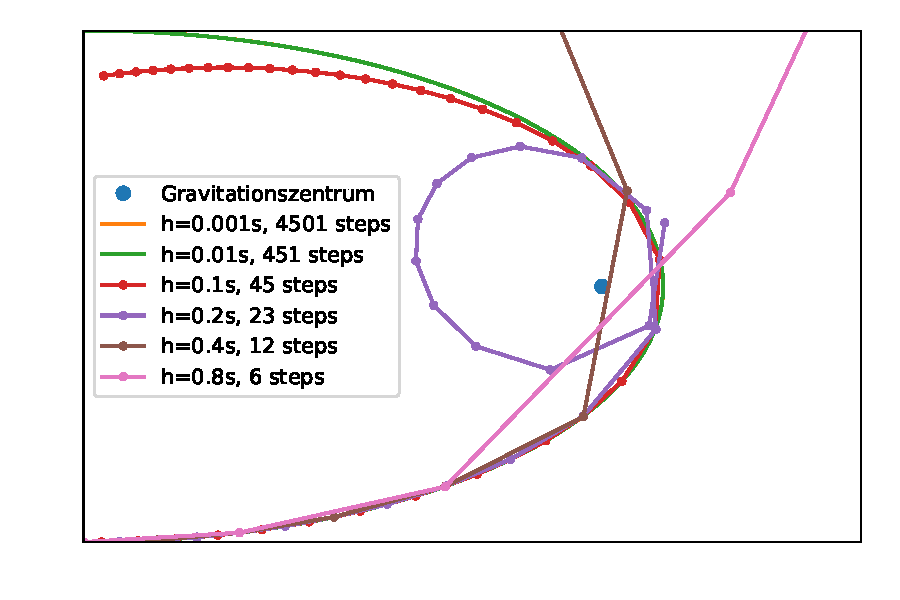
\includegraphics[width=0.5\textwidth]{papers/steps/img/gravity_different_fixed_stepsize.pdf}
\caption{Bahn eines Teilchens, von unten links kommend,
um ein Gravitationszentrum, berechnet mit unterschiedlichen Schrittweiten (Runge-Kutta 4. Ordnung):
$a(t)=P''(t)=\frac{(Pfix-P(t))\cdot m\cdot g}{|Pfix-P(t)|^{3}}$
mit $P(0)=(0, 0)$, $Pfix(2, 1)$, $P'(0)=v(0)=(0.669, 0)$, $g=1$, $m=1$
\label{buch:steps:fixed_comparison}}
\end{figure}

Welche Wirkung verschiedene Schrittgrössen
auf das Resultat haben können, wird in Grafik~\ref{buch:steps:fixed_comparison} gezeigt.
In dieser Grafik ist auch ersichtlich, dass fernab dem Gravitationszentrum auch grössere Schritte
ausreichende Genauigkeit liefern und die kleinen Schritte somit nur in der Nähe des Gravitationszentrums
nötig sind, wo die Geschwindigkeit und die Beschleunigung gross ist.

%\ref{steps:section:folgerung}.



